\documentclass{beamer}
\usepackage{animate}
\usepackage{graphicx}
\usepackage{pgffor}
\usepackage[T1]{fontenc}
\usepackage{amsmath}
\usepackage[utf8]{inputenc}
\usepackage[german]{babel}
\usepackage[scaled]{helvet}
\usepackage{minted}
%\renew{\familydefault}{\sfdefault}
\usepackage{markdown}
\usepackage{blindtext}
\usepackage{adjustbox}
\usepackage{calc}
\usepackage{listings}
\usepackage{xcolor}
\usepackage{geometry}
\usepackage{longtable}
\usepackage{array}
\usepackage{tabularx}
\usepackage{hyperref,graphicx}
\usepackage{caption}
\usepackage{refstyle}
\usepackage{pdfpages}
\usepackage{comment}
\usepackage{listings}
%\usepackage{xcolor}
%\graphicspath{{bilder/}}
\usepackage{import}
%\usepackage[dvipsnames,table]{xcolor}
%\usepackage{hyperref}
%\us^epackage{multirow}
%\usepackage{textpos}
\usepackage{listings}
\usepackage{color}
\usepackage{tikz}
\usepackage{pgfplots}
\usepackage{ragged2e}
\usepackage{blindtext}
\usepackage{lmodern}
\usepackage[framemethod=tikz]{mdframed}
\usepackage{fixltx2e}
\usepackage{textcomp}
\usepackage{textpos}
\usepackage{tikz}
\usepackage{etoolbox}
\def\code#1{\texttt{#1}}

\definecolor{darkgreen}{RGB}{0, 100, 0}

\hypersetup{
	colorlinks=magenta,
	linkcolor=blue,
	filecolor=magenta,
	urlcolor=cyan,
	pdftitle={Overleaf Example},
	pdfpagemode=FullScreen,
}

\usetheme{Antibes}
    \setbeamertemplate{footline}[page number]
    \setbeamercovered{transparent=25}
  \setbeamertemplate{navigation symbols}{}
\usecolortheme{dolphin}

\setbeamercolor{item}{fg=cyan}
%\setbeamercolor{section in toc}{fg=cyan}
\setbeamercolor{alerted text}{fg=cyan}
\setbeamercolor{block title}{bg=blue, fg=white}
\setbeamercolor{block body}{bg=lightgray, fg=black}
\definecolor{myblue}{RGB}{0, 102, 104}

\title{Funktionale Programmierung}

%\titlegraphic{
%
\includegraphics[scale=0.1]{nix-snowflake.svg}
%}
\author{Thanh Viet Nguyen}
%\institute[]{Hochschule Hannover}


\begin{document}
\begin{frame}%[plain]
    \maketitle
    \centering
 
\includegraphics[scale=0.15]{bilder/hsh-logo.jpg}[h]
   \date{09.12.2024}

\end{frame}

\begin{frame}
	\tableofcontents
\end{frame}


\section{Einleitung}
\begin{frame}
\begin{itemize}
\item Was ist ein Funktionale Programmierung?
\item Historische Entwicklung und Ursprung.
\item Unterschiede zur imperativen Programmierung
\item Wichtige Konzepte: Funktionen als erste Klasse, Unveränderlichkeit und Rekursion
\item Praktische Beispiele
\item Ziel der Präsentation: Verständnis der Grundlagen und praktischen Anwendungen der funktionalen Programmierung.

\end{itemize}
\end{frame}


\section{Herkunft der Funktionalen Programmierung}
\begin{frame}

	\begin{itemize}
		\item Lambda Kalkül (1930): Alonzo Church (14.06.1903 - 11.08.1995)
		\item Vor Maschinen, die solchen Code ausführen konnten, gab es bereits Ansätze dazu.
            \item Typen Theorie
	\end{itemize}

\end{frame}

\section{Programmier Paradigmen Übersicht}
\begin{frame}
	\begin{figure}
	    \centering
	    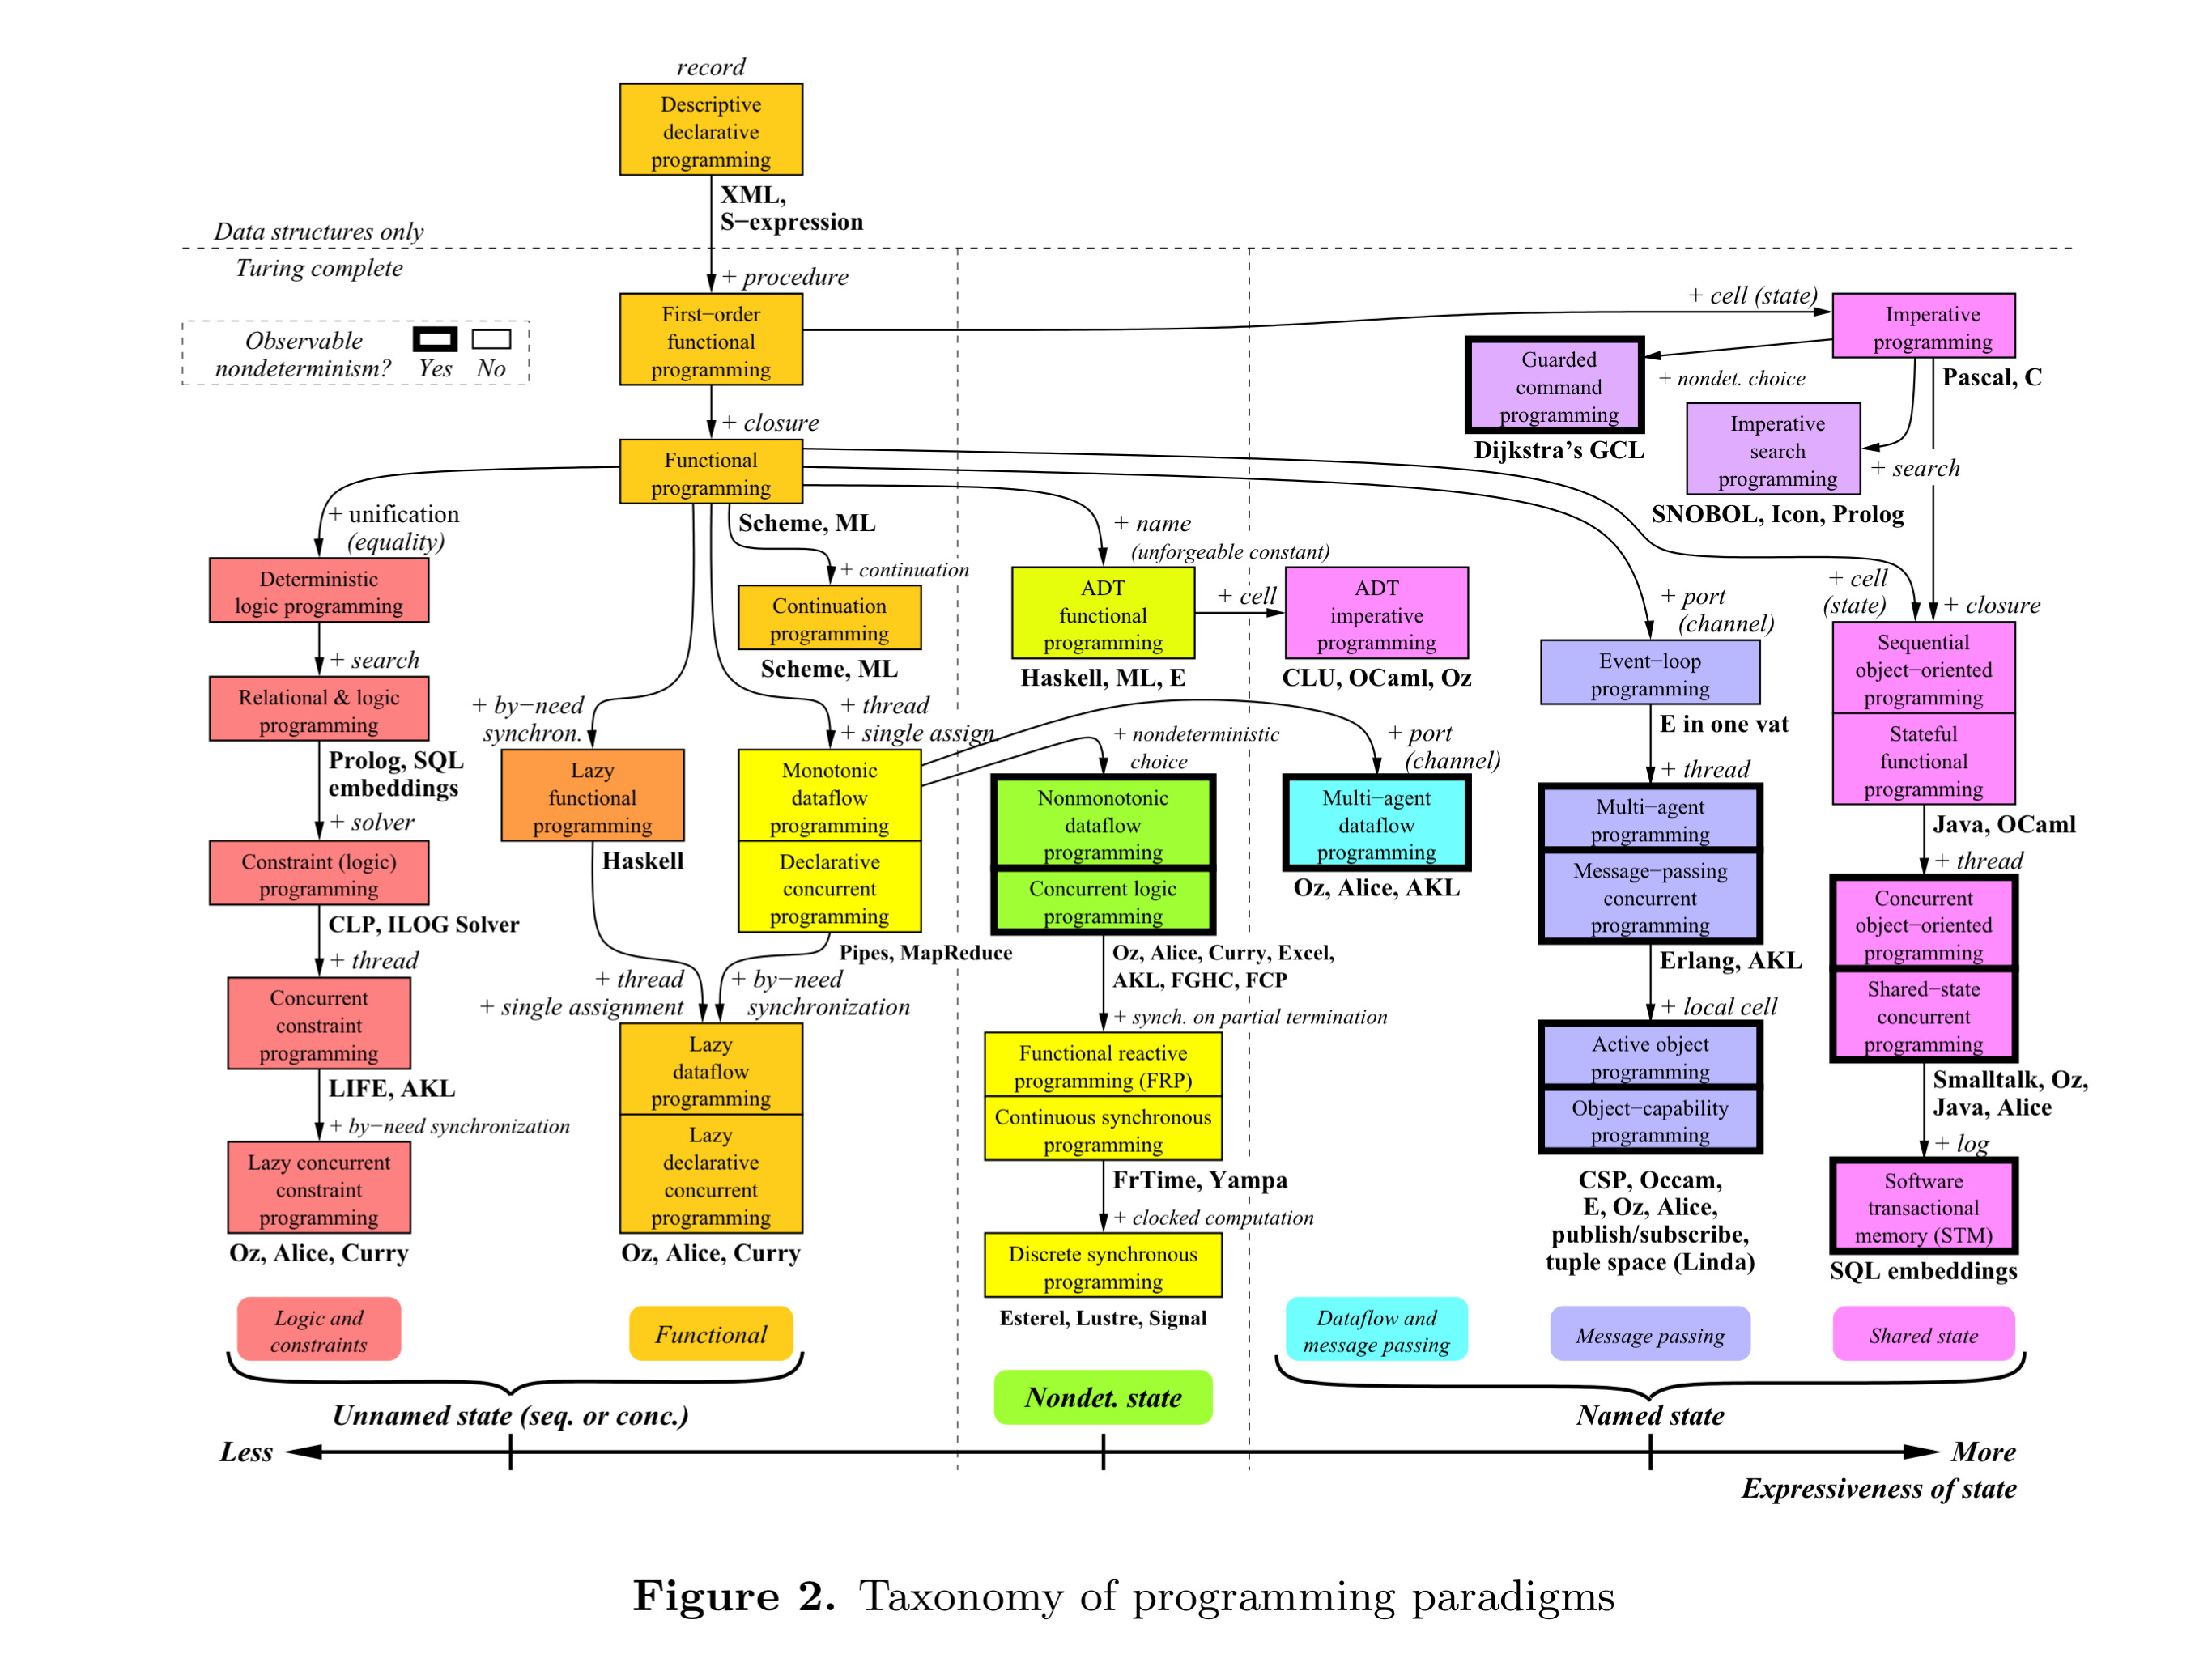
\includegraphics[width=0.9\linewidth]{bilder/Programming-paradigms.png}
	    \textmd{ \tiny https://blog.acolyer.org/2019/01/25/programming-paradigms-for-dummies-what-every-programmer-should-know/}
	    %\label{fig:enter-label}
	\end{figure}
\end{frame}

\begin{frame}{Objekt Orientierung und Funktionale Programmierung}
\begin{figure}
    \centering
    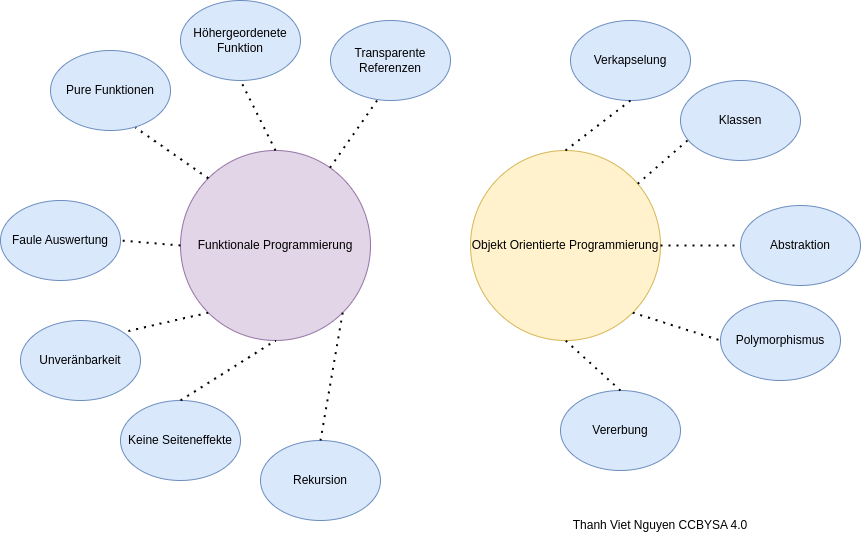
\includegraphics[scale=0.38]{bilder/Unterschiede.drawio.png}
\end{figure}

\end{frame}

\begin{frame}{Deklaritive und Imperativen Programmiereung}
\centering
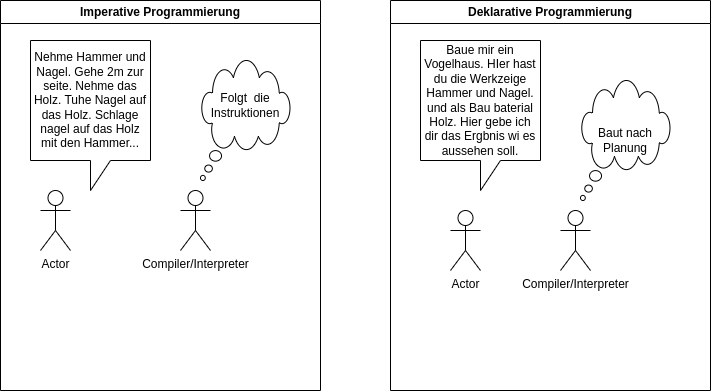
\includegraphics[scale=0.38]{bilder/ProgrammierParadigmen.drawio.png}

\end{frame}

\begin{frame}

    \url{https://xkcd.com/435/}
\end{frame}

\subsection{Lambda Kalkül}
\begin{frame}
	\begin{itemize}
 %alonzo church
	    \item Formales System in der Mathematik für Aussagen bearbeitung
            \item
	\end{itemize}
	%$"quadrat_summe"(x_y) = x^2 + y^2$ akk
\end{frame}

\begin{frame}[Turing Vollstäntdigkeit]

\textmd{Turing Machine: Ein theoretisches Modell, das als Grundlage für die Berechenbarkeit dient. Es besteht aus einem unendlichen Band, einem Lese-/Schreibkopf und einer endlichen Zustandsmenge.}

\textmdE{in System ist Turing-vollständig, wenn es in der Lage ist, jede berechenbare Funktion auszuführen, die ein Turing-Maschine ausführen kann.}


\end{frame}

\begin{frame}
\frametitle{Lisp Maschinen}
	\begin{itemize}
            \item 1960er
            \item Erforschung von Künstlicher Intelligenz
	\end{itemize}

\end{frame}

\begin{frame}
\frametitle{Lisp Dialekte}
	\begin{figure}
	    \centering
	    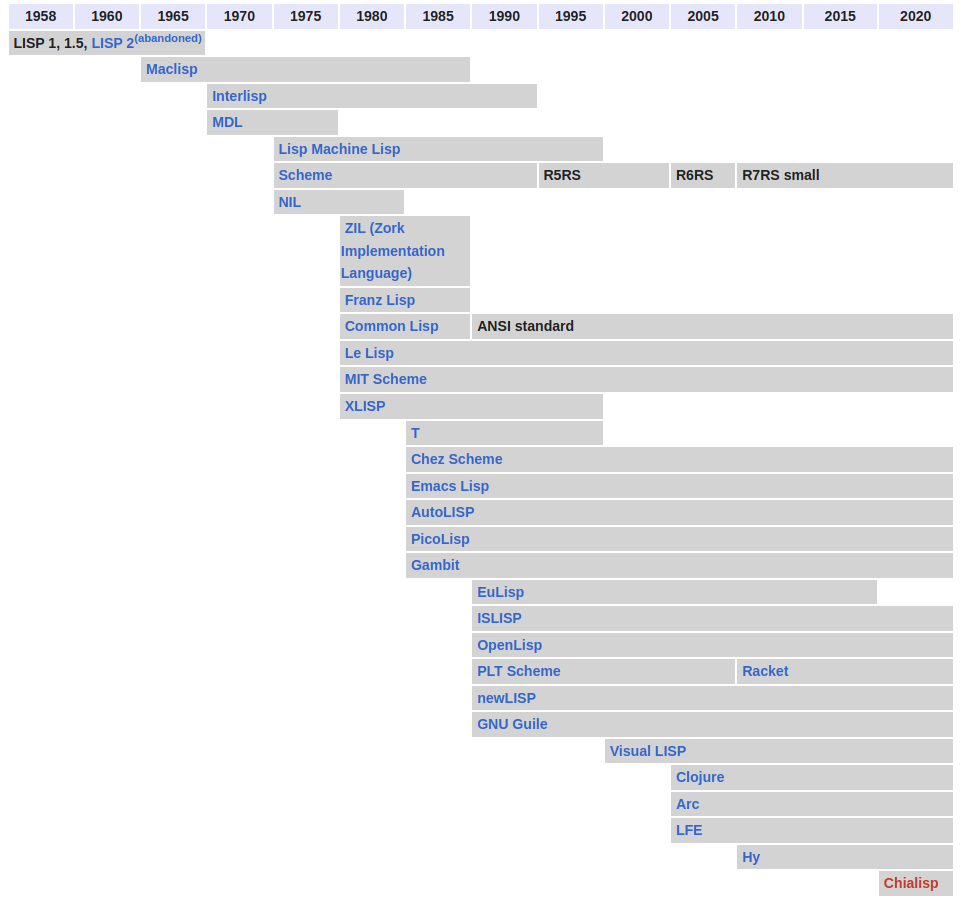
\includegraphics[width=0.7\linewidth]{lisphis.png}
            \textmd{ \tiny \url{https://en.wikipedia.org/wiki/Lisp_(programming_language)}}
	    %\caption{Enter Caption}
	    %\label{fig:enter-label}
	\end{figure}
\end{frame}



\begin{frame}
	\begin{figure}
	    \centering
	    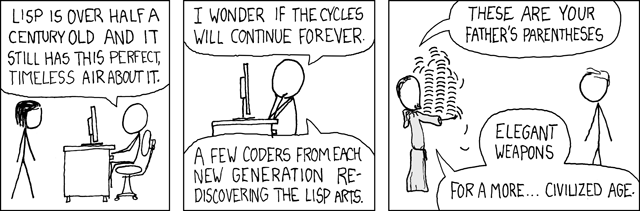
\includegraphics[width=1\linewidth]{bilder/lisp_cycles.png}
        \textmd{ \tiny \url{https://www.explainxkcd.com/wiki/index.php/297:_Lisp_Cycles}}
	    %\caption{Enter Caption}
	    %\label{fig:enter-label}
	\end{figure}
\end{frame}


\section{Features der Funktionalen Programmierung}
\begin{frame}
	\begin{itemize}
		\item Fokus auf unveränbare Daten
            \item Wenn eine Funktion pur ist, folgt: \code{Kein State -> keine Seiteneffekte}
            \item Basiert sich auf Aussagen
            \item Rerefrenzen sind Transparent:   \code{input -> output}
	\end{itemize}
\end{frame}


\begin{frame}
\frametitle{Zusätzliche Konzepte }
	\begin{itemize}
			\item Currying: Umwandlung von Funktionen, die mehrere Argumente annehmen, in eine Kette von Funktionen, die jeweils ein Argument akzeptieren.
			\item Functor: \begin{itemize}
			    \item Functor: Beschreibt, wie Funktionen mit "fmap",  auf Werte in einem bestimmten Zusammenhang angewendet werden.
                    \item  Befolgt Identitätsregel und Kompositionsregel.
			\end{itemize}
                \item Applificat: \begin{itemize}
                    \item Verwendet die Funktionen   "pure" oder "return", um Werte in den Kontext zu bringen
                    \item Nutzt den Operator ">>=" , um Berechnungen zu verknüpfen
                    \item Befolgt Identitäts- und Assoziativitätsregeln.
                \end{itemize}
                \item Monad: \begin{itemize}
                    \item Verknüpft Berechnungen in einem Kontext.
                    \item Definiert durch "return" oder "pure" und ">>=" (Bind).
                    \item Befolgt Identitätsregel und Assoziativitätsregel.
                \end{itemize}
	\end{itemize}

\end{frame}

\begin{frame}{Currying}

 \begin{figure}
     \centering
     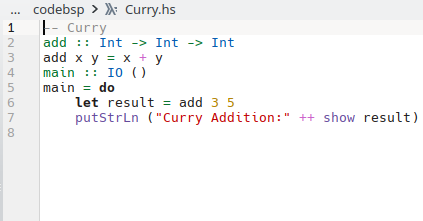
\includegraphics[scale=0.5]{bilder/FP-Curry-hs.png}
 \end{figure}
 \begin{figure}
     \centering
     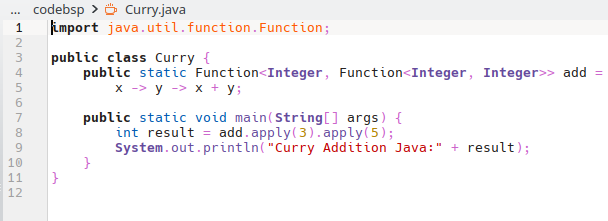
\includegraphics[scale=0.5]{bilder/FP-Curry-java.png}
 \end{figure}

\end{frame}

\begin{frame}
\frametitle{Functor}

 \begin{figure}
     \centering
     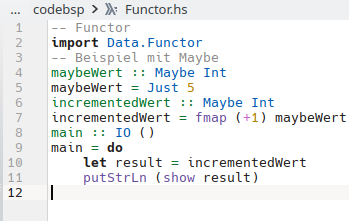
\includegraphics[scale=0.5]{bilder/FP-Functor-hs.png}
 \end{figure}
 \begin{figure}
     \centering
     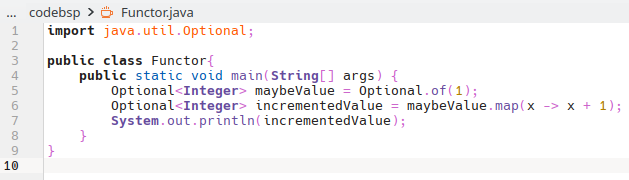
\includegraphics[scale=0.5]{bilder/FP-Functor-java.png}
 \end{figure}

\end{frame}

\begin{frame}
\frametitle{Applicative}
 \begin{figure}
     \centering
     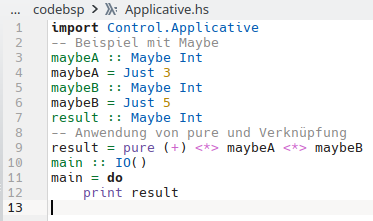
\includegraphics[scale=0.5]{bilder/FP-Applicative-hs.png}
 \end{figure}
 \begin{figure}
     \centering
     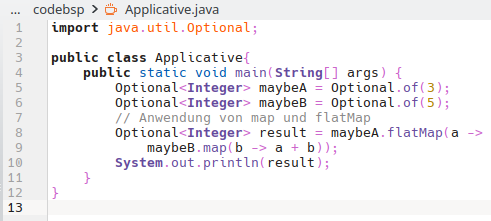
\includegraphics[scale=0.5]{bilder/FP-Applicative-java.png}
 \end{figure}
\end{frame}

\begin{frame}
\frametitle{Monad}

  \begin{figure}
     \centering
     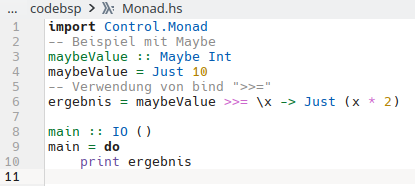
\includegraphics[scale=0.5]{bilder/FP-Monad-hs.png}
 \end{figure}
 \begin{figure}
     \centering
     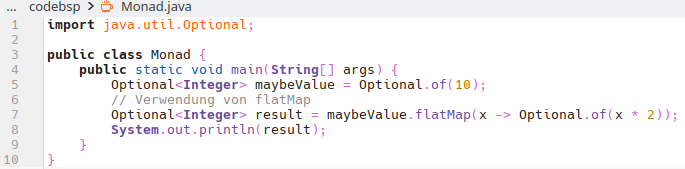
\includegraphics[scale=0.5]{bilder/FP-Monad-java.png}
 \end{figure}

\end{frame}


\section{Vorteile und Nachteile}
\begin{frame}
\centering
	\begin{tabular}{ |p{5cm}|p{5cm}|  }
		\hline
             \textcolor{darkgreen}{Vorteile} & \textcolor{red}{Nachteile} \\
		\hline
		Mehr Sicherheit beim Entwickeln: Nebenläufigkeit, Wartbarkeit, und Testbarkeit & Kein Zustand -> Keine Zustandskontrolle \\
            \hline
            Modularität & \\
            Paralelle Verarbeitung& \\
		\hline
            Mehr Speichersicherheit  & meist Speicher intensiver bei der Laufzeit  \\
		\hline
    Code ist in der Regel lesbarer und Kürzer & Lesbarkeit \neq Verständlich \\
            Höhere Abstraktion & \\
		\hline

 \end{tabular}

\end{frame}

\section{Anwendungsgebiete}
\begin{frame}
	\begin{itemize}
            \item Software Anwendungen (Webanwendung, Desktopanwendungen, Services, etc.)
            \begin{itemize}
            \item  Sicherstellung von Software
            \end{itemize}
		\item Systemkonfigurationen
		\item Beweisasistent für Mathematische Theoreme
            \item Verarbeitung von Forschungsdaten
    \end{itemize}
\end{frame}

\begin{frame}{Beweisassistent für Theoreme}
\centering
    \begin{itemize}
        \item  Roqc \text{für Lisp Dialekt Liebhaber}
        \item  Lean \text{für nicht Lisp Dialekt Liebhaber}
    \end{itemize}

\end{frame}

\begin{frame}
\frametitle{Deklarative Systemkonfigurationen und Reproduzierbare Bauten}
 \begin{itemize}
		\item NixOS: GNU/Linux Distro
		\item Guix: GNU/Linux Distro, welches mit Guile Scheme Dialekt Konfiguriert wird
		\item Emacs: Ein Texteditor mit vielen erweiterungen, welches mit Lisp Dialekt (Elisp)
		\item Debian GNU/Linux verwendung von OCAML für Reproduzierbare Checks
            \item Code als Basis für Infrastrukturen
\end{itemize}

\end{frame}

\begin{frame}
    \begin{figure}
    \centering
    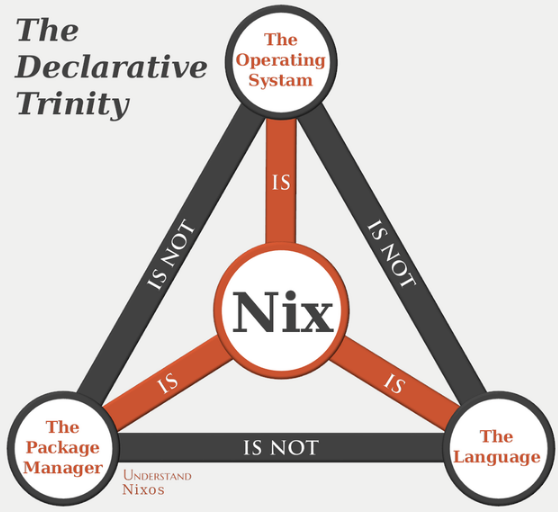
\includegraphics[width=0.7\linewidth]{bilder/nix.png}
    \textmd{\tiny \url{https://github.com/gytis-ivaskevicius/high-quality-nix-content/tree/master/memes} }
    %\caption{Caption}
    %\label{fig:enter-label}
\end{figure}

\end{frame}

\section{Fazit}
\begin{frame}
	\begin{itemize}
		\item Grundverständnis zur Funktionalen Programmiereung
		\item Lambda Kalkulus etwas kennen gelernt
		\item Schwächen und Stärken der Funktionalen Programmierung
            \item Anwendungsgebiete die von FP geführt werden
            \item Wird in der Zukunft häufiger verwendet durch Entwickeln mit KI und Quantencomputer
            \item FP ist nicht die Lösung für alle Probleme in der Softwareentwicklung.
            %\item \textmd{$\neg \forall x \, (\text{Lösung}(x) \rightarrow \text{funktionale Programmierung}(x)) \land \exists y \, (\text{optimale Lösung}(y) \land \text{Problem}(y) \land \text{funktionale Programmierung}(y))$}
            %\item $\neg \forall \times ( Lösung(x) \rightarrow y(\text{FunktionaleProgrammierung}(x)) \and \exists y(\text{OpitimaleLösung}(y)) \and \text{Problem}(y) \and \text{FunktionaleProgrammierung}(y)) $ .

        \end{itemize}
\end{frame}

\begin{frame}
\centering
\frametitle{Mehr erfahren? \\ Hier sind einige Einsteiger freundliche Projekte}
\begin{itemize}
    \item FP für weitere Programmier Sprachen: \url{https://learnfp.org/}
    \item Mehr über Haskell:\url{https://learnyouahaskell.github.io/}
    \item Falls jemand nicht genug hat: \url{https://nixos.org/learn/}
    \item \code{(defun display-message () \\
  (let ((message "Falls jemand immer noch nicht genug hat: \url{https://guix.gnu.org/cookbook/}"))
(display-message)))}


\end{itemize}

\end{frame}

\begin{frame}
	\section{Quellen}
	\begin{itemize}
		\item \url{https://achimjungbham.github.io/pub/papers/lambda-calculus.pdf}
		\item  \url{https://hackmd.io/@9LWWQ7ZlTjK0WMATI1lXgg/HkDzV88Sp} %{Nixified BBB}
		\item \url{https://en.wikipedia.org/wiki/Lambda_calculus}
            \item \url{https://bitsavers.org/pdf/mit/cadr/chinual_6thEd_Jan84/}
            \item \url{https://www.mdc-berlin.de/research/publications/pigx-reproducible-genomics-analysis-pipelines-gnu-guix}
	\end{itemize}
 \centering
 \textbf{Literatur}
 \begin{itemize}
     \item Mathematics
in Programming (Xinyu Liu)
\item Functional and
Logic Programming (Gerhard Goos, Juris Hartmanis)
\item $\text{Revised}^6$ Report on the Algorithmic Language
Scheme ()
 \end{itemize}
\end{frame}


\end{document}
